\clearpage
\section{TX-side LO Suppression}
\label{sec:lo-suppression}
% numbers: sections/sec6_cal_numbers.tex (100 MHz-grid calibration, cold + hot), loaded in the Key Specifications section
% (quoted there first)
% generated by FR3_Characterization/plot_datasheet_lo_cal.py -- do not edit
\newcommand{\tdiffMedianMv}{4}
\newcommand{\tdiffNinetyMv}{8}
\newcommand{\tdiffMaxMv}{36}
\newcommand{\nullRiseOneMv}{27}
\newcommand{\nullRiseThreeMv}{36}


\textbf{Inside a quadrature mixer.} Figure~\ref{fig:6-qmix} shows how a quadrature mixer works as an up-converter.
It has four ports: the I and Q inputs, the LO input, and the RF output. Inside, a 90-degree hybrid splits the LO into
two copies a quarter of a cycle apart: the in-phase LO (0 degrees) and the quadrature LO (90 degrees). The I-mixer
multiplies the I input by the in-phase LO, the Q-mixer multiplies the Q input by the quadrature LO, and the two products
are summed at the RF port. An ideal mixer would output only the wanted sideband; a real one also leaks some of each LO
copy into that sum.

\begin{center}
\begin{tikzpicture}[
  port/.style={draw, circle, fill=black, inner sep=1.2pt},
  mixer/.style={draw, circle, minimum size=8mm, inner sep=0pt, fill=blue!10, font=\large},
  sum/.style={draw, circle, minimum size=7mm, inner sep=0pt, fill=gray!8, font=\large},
  hyb/.style={draw, rectangle, minimum width=1.7cm, minimum height=0.9cm, align=center, font=\scriptsize, fill=gray!8},
  arr/.style={-{Stealth[length=2mm]}, thick},
  leak/.style={-{Stealth[length=1.8mm]}, thick, red!75!black, densely dashed},
  lbl/.style={font=\scriptsize, align=center}
]
\node[port] (iin) at (0, 1.7) {};
\node[port] (qin) at (0, -1.7) {};
\node[port] (loin) at (0, 0) {};
\node[lbl, left=1mm of iin] {I in};
\node[lbl, left=1mm of qin] {Q in};
\node[lbl, left=1mm of loin] {LO in};
\node[mixer] (mi) at (4.2, 1.7) {$\times$};
\node[mixer] (mq) at (4.2, -1.7) {$\times$};
\node[hyb] (hy) at (4.2, 0) {90$^\circ$ hybrid\\splitter};
\node[sum] (sm) at (7.4, 0) {$+$};
\node[port] (rfout) at (9.6, 0) {};
\node[lbl, right=1mm of rfout] {RF out};
\node[lbl, above=0.5mm of mi] {I-mixer};
\node[lbl, below=0.5mm of mq] {Q-mixer};
\draw[arr] (iin) -- (mi);
\draw[arr] (qin) -- (mq);
\draw[arr] (loin) -- (hy);
\draw[arr] (hy) -- node[lbl, right] {in-phase LO (0$^\circ$)} (mi);
\draw[arr] (hy) -- node[lbl, right] {quadrature LO (90$^\circ$)} (mq);
\draw[arr] (mi) -| (sm);
\draw[arr] (mq) -| (sm);
\draw[arr] (sm) -- (rfout);
\node[lbl, text=red!75!black, anchor=south west, align=left] at (4.8, 1.72) {I product\\+ LO leaked by the I-mixer};
\node[lbl, text=red!75!black, anchor=north west, align=left] at (4.8, -1.72) {Q product\\+ LO leaked by the Q-mixer};
\draw[densely dotted, gray] (1.4, -2.75) rectangle (8.2, 2.75);
\node[lbl, gray, anchor=north east] at (8.2, 2.75) {quadrature mixer};
\end{tikzpicture}
\captionof{figure}{A quadrature mixer used as an up-converter. The 90-degree hybrid splits the LO into an in-phase
copy, mixed with the I input, and a quadrature copy, mixed with the Q input; the two products are summed at the RF
output. Each mixer's output also carries some LO that the mixer leaks (red), so the LO leakage at
the RF output is the sum of what the two mixers leak.}\label{fig:6-qmix}
\end{center}

\textbf{What causes LO leakage, and why it matters.} The LO that each of the two mixers leaks into its output adds
up to a tone at the LO frequency at the RF port: the LO leakage. It does real harm. It is a strong, constant tone that
takes up output headroom in the amplifiers after the mixer, whatever is being transmitted, and a strong enough one can
drive the final amplifier into compression on its own. It also mixes with the transmitted signal in those amplifiers
(Section~\ref{sec:compression-upper}), and some of the resulting products land on the unwanted sideband,
worsening the sideband suppression of Section~\ref{sec:sideband-suppression}. And it puts real RF power at a frequency
the unit was never asked to transmit.

\textbf{A secondary source of LO leakage.} The LO is a strong signal inside the unit, and not all of the LO that
reaches the ``TX-side FR3 RF Out'' connector comes out of the mixer through the AM3153 filter. A small part reaches the
output by other paths that do not go through the filter. We see it directly in the measurements: in filter settings
that attenuate the LO frequency by 40\,dB or more, the LO leakage at the connector is no lower than in settings that
pass it. Because this part does not depend on the filter setting, it sets a floor under the LO leakage that no filter
setting can remove.

\textbf{How the bias cancels LO leakage.} Any DC voltage on the mixer's I and Q inputs also comes out at the LO
frequency. So a deliberate DC bias on those two lines --- two voltages this unit calls I\_V and Q\_V --- can be set to
produce a tone of the same size and opposite phase, cancelling the LO leakage. Plotted against I\_V and Q\_V, the
leakage power forms a smooth bowl with one minimum, and a search finds it: starting from I\_V~=~Q\_V~=~0\,V, it steps
on the I and Q axes, moves to whichever neighbouring point reads lowest, and halves the step whenever no neighbour is
lower. Once close to the bottom, a few nearby readings are used to fit the bowl's shape, and the minimum of that fit is
the nulled bias. Because the search minimizes the leakage measured at the ``TX-side FR3 RF Out'' connector, the bias it finds suppresses the total LO leakage at that output port, from both sources (the mixer and the secondary source), in the configuration the search was run in.

\textbf{Two sources, a very large search space.} For any one configuration --- a 5-dimensional search space of (FR1, FR3, sideband, filter setting, and temperature)
--- a search run in exactly that configuration finds the bias that cancels the \emph{total} LO leakage, from both
sources at once. But there are far too many configurations to calibrate each unit at the factory. The calibration
therefore makes one search per LO frequency (\calLoCount{} LO frequencies), in a single \emph{reference} filter setting,
at two different temperatures. The reference setting is, of the settings that can be in use at that LO frequency, the
one that passes the LO frequency with the least loss. There the mixer's leakage is
much stronger than the secondary leakage, so the null found there cancels the mixer's leakage. That one bias pair is
then used with every filter setting at that LO frequency: it keeps cancelling the mixer's leakage, but the secondary
leakage is not cancelled and comes through as it is. In most filter settings, the floor it sets is what is left. The
same bias pair serves both sidebands: we tested both, and the LO leakage did not change in any meaningful way between
them (the only changes were in readings already far below the \calThreshold\,dBm threshold).

\textbf{Factory calibration and temperature.} The bias that cancels the mixer's leakage drifts with temperature, and it
differs from unit to unit because it depends on each unit's own small circuit mismatches. Every unit is therefore
calibrated individually, on a 100\,MHz grid of LO frequencies from 7.0 to 22.5\,GHz (\calLoCount{} LO frequencies), at
two temperatures. FR1 and FR3 are chosen as multiples of 100\,MHz, so the LO always lands on a calibrated grid point.
Each LO frequency is calibrated at the LO drive it uses (\lmxDriveRule). The temperature is the LMX2820 synthesizer's
die temperature, from its built-in sensor: the ``cold'' calibration is made with the die at
\calColdMinC--\calColdMaxC\textdegree C and the ``hot'' one at \calHotMinC--\calHotMaxC\textdegree C. The unit's flash
stores one (I\_V, Q\_V) pair per LO frequency for each temperature (Figure~\ref{fig:6-3}), each with the die
temperature it was measured at. At runtime the unit applies it by itself: on every tune, and again every 2\,seconds,
its firmware reads the die temperature and interpolates between the cold and hot values (or extrapolates beyond them),
and sets the bias. Setting I\_V or Q\_V by hand switches this off; \texttt{IQBIAS AUTO} switches it back on
(Appendix~\ref{sec:commands}). The two temperatures matter because the null is very narrow. Between the cold and the hot calibration the stored bias moves by a median of \tdiffMedianMv\,mV (90\% of LO frequencies: \tdiffNinetyMv\,mV or less; up to \tdiffMaxMv\,mV), Figure~\ref{fig:6-4}, while in the reference setting a bias just 1\,mV off the null already raises the LO leakage by about \nullRiseOneMv\,dB, and 3\,mV off by about \nullRiseThreeMv\,dB. Using the cold bias on a hot unit, or the other way round, would therefore throw away most of the suppression; interpolating between the two tables by temperature keeps it. One
temperature's calibration takes about \calMinutesPerTemp{} minutes.\footnote{Disclaimer: these factory values are a
snapshot of the unit's behavior at calibration time; because they depend on small analog mismatches, they can change
over time, so a calibration should not be assumed valid indefinitely.}

\textbf{Pass criterion.} At each temperature, the calibration re-measures the LO leakage in every filter setting at
every LO frequency: \calReadCount{} readings, one per (LO frequency, filter setting) pair. It passes when at least
\calPassPct\% of them are at or below \calThreshold\,dBm at the ``TX-side FR3 RF Out'' connector.

\textbf{What you get.} Figures~\ref{fig:6-1} and~\ref{fig:6-1h} show the LO leakage after the cold and the hot
calibration. Read them one LO frequency at a time: the line is the median across the filter settings usable at that LO
frequency, and the shaded band spans the best setting to the worst. Where the top of the band stays below the dashed
\calThreshold\,dBm line, every setting passes. The reference setting is left out: the leakage there is far lower than in
any other setting (median \calRefMedian\,dBm). Figure~\ref{fig:6-2} shows all the readings as histograms. In the cold
calibration, \calColdPct\% of the readings are at or below \calThreshold\,dBm (median \calColdMedian\,dBm, worst
\calColdWorst\,dBm); in the hot calibration, \calHotPct\% (median \calHotMedian\,dBm, worst \calHotWorst\,dBm).

\textbf{Your unit will differ --- and you can do better yourself.} On your own unit, Figure~\ref{fig:6-1} may look quite
different: the leakage drifts, and one stored bias pair per LO frequency has to serve every filter setting. If LO
leakage matters for your experiment, set the unit up exactly as your experiment uses it (the same FR1, FR3, sideband, and filter setting), run the search described above on the LO leakage at the ``TX-side FR3 RF Out'' connector, and set
the result with the \texttt{SET I\_V} and \texttt{SET Q\_V} commands (Section~\ref{sec:commands}), which also
switch the automatic bias off, so it stays put. In that one
configuration, the search cancels the total LO leakage, including the secondary leakage that the factory calibration
leaves in place.

\clearpage
% the three LO-suppression figures together on one page, each in its own full-width row (user layout, 2026-10-05)
\begin{center}\begin{minipage}{\linewidth}\centering% graphic and caption kept together
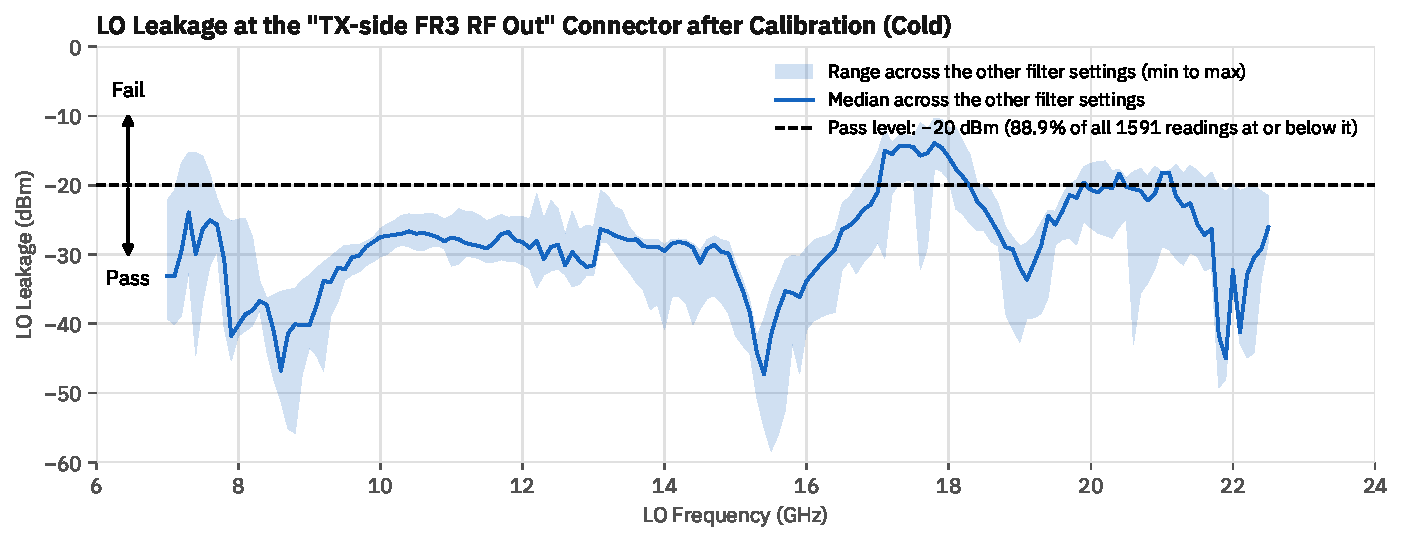
\includegraphics[width=\linewidth]{images/sec6_cal_fig1.pdf}
\captionof{figure}{LO leakage at the ``TX-side FR3 RF Out'' connector after the cold calibration, at each of the
\calLoCount{} calibrated LO frequencies (100\,MHz steps). At each LO frequency, the stored bias pair was applied and
the LO leakage was measured in every filter setting that can be in use at that LO frequency, other than the
reference setting the null was found in. The line is the median of those readings, and the shaded band spans the
lowest to the highest of them. The dashed line is the \calThreshold\,dBm pass level.}\label{fig:6-1}
\end{minipage}\end{center}
\vspace{-0.8em}
\begin{center}\begin{minipage}{\linewidth}\centering% graphic and caption kept together
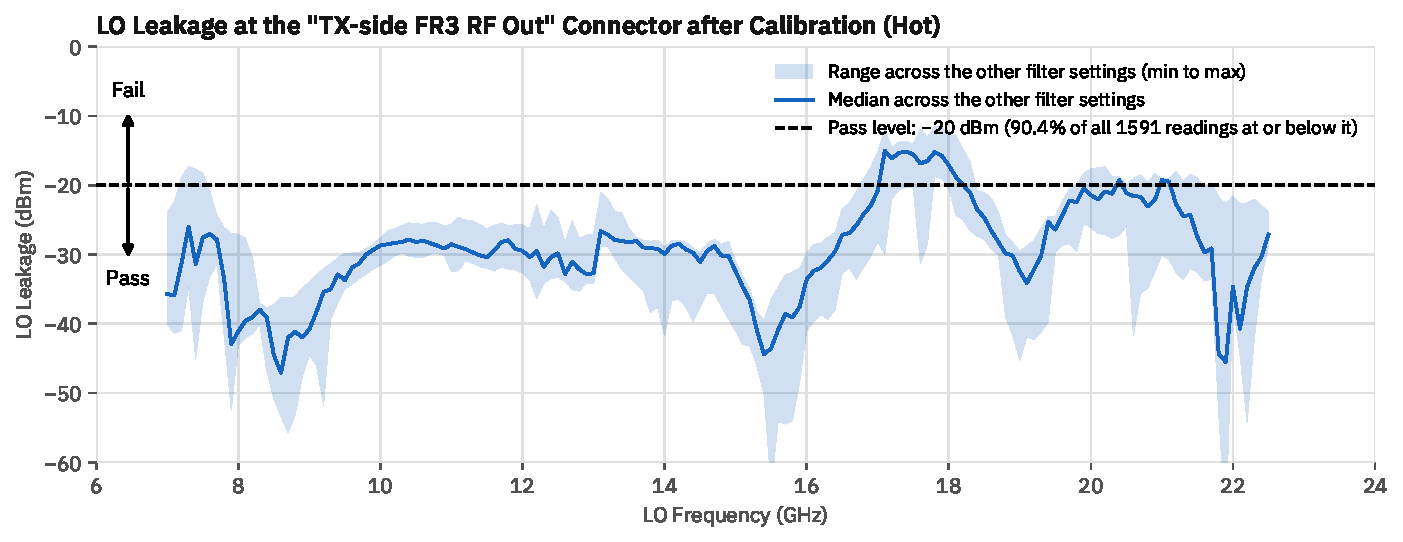
\includegraphics[width=\linewidth]{images/sec6_cal_fig1_hot.pdf}
\captionof{figure}{The same as Figure~\ref{fig:6-1}, after the hot calibration (LMX die at
\calHotMinC--\calHotMaxC\textdegree C).}\label{fig:6-1h}
\end{minipage}\end{center}
\vspace{-0.8em}
\begin{center}\begin{minipage}{\linewidth}\centering% graphic and caption kept together
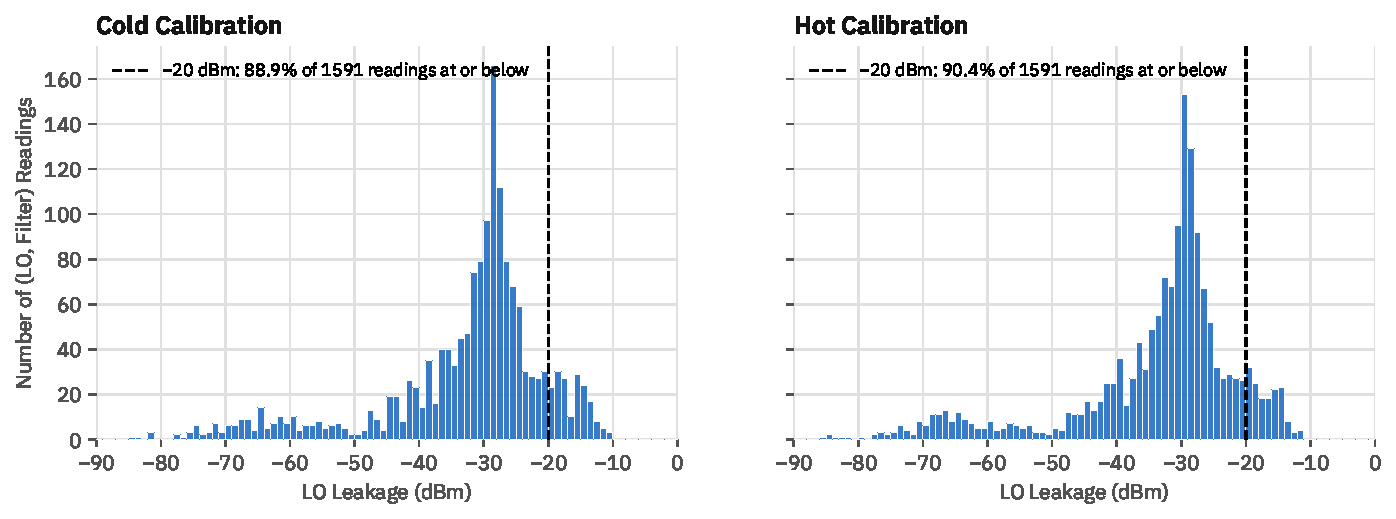
\includegraphics[width=\linewidth]{images/sec6_cal_fig2.pdf}
\captionof{figure}{All the readings of the cold and the hot calibration as histograms: the number of (LO frequency, filter setting)
readings, the reference setting included, at each level of LO leakage, in 1\,dB bins. The dashed line is the
\calThreshold\,dBm pass level; a calibration passes when at least \calPassPct\% of the readings are at or below
it.}\label{fig:6-2}
\end{minipage}\end{center}
\vspace{-0.8em}
\begin{center}\begin{minipage}{\linewidth}\centering% graphic and caption kept together
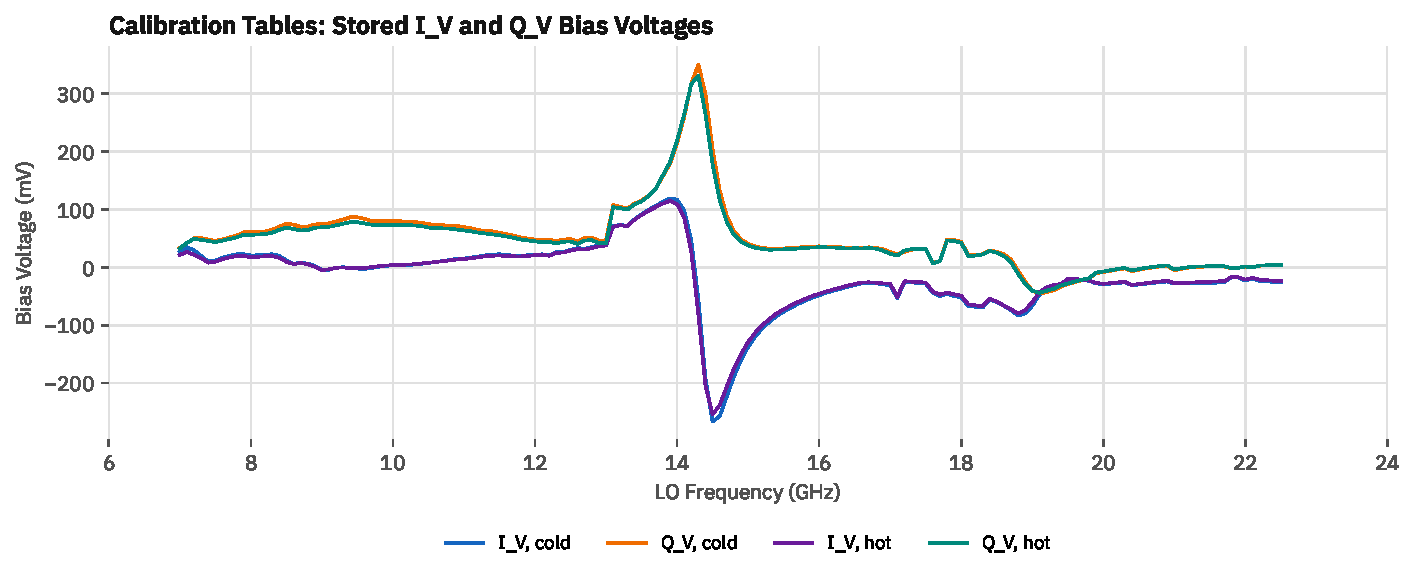
\includegraphics[width=\linewidth]{images/sec6_cal_fig3.pdf}
\captionof{figure}{The unit's two calibration tables: at each LO frequency (100\,MHz steps), the I\_V and Q\_V bias
voltages stored in flash. Cold: recorded with the LMX die at \calColdMinC--\calColdMaxC\textdegree C. Hot: recorded
with the LMX die at \calHotMinC--\calHotMaxC\textdegree C. At runtime the bias is interpolated between
these.}\label{fig:6-3}
\end{minipage}\end{center}
\vspace{-0.8em}
\begin{center}\begin{minipage}{\linewidth}\centering% graphic and caption kept together
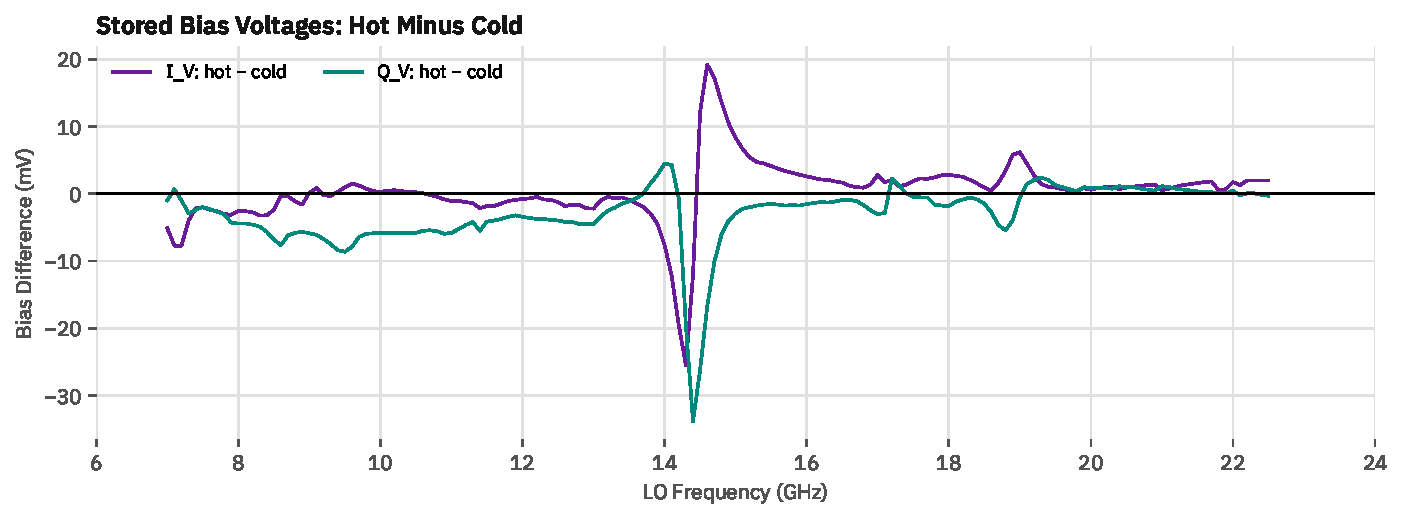
\includegraphics[width=\linewidth]{images/sec6_cal_fig4.pdf}
\captionof{figure}{The difference between the two calibration tables of Figure~\ref{fig:6-3}: hot minus cold, for I\_V and Q\_V, at each LO frequency. A few mV is enough to change the LO leakage by tens of dB, which is why the bias is interpolated by temperature at runtime.}\label{fig:6-4}
\end{minipage}\end{center}
